% I've played with the wording of Macej's article a little, and particularly removed a few articles and elipsis.
On your way in, you should have been assigned to one of three teams - the Rebels, the Pioneers, or the Companions
- and given a sticky badge to wear with newfound pride.
If somehow you slipped through the net,
or misplaced your badge,
then go and \emph{politely} berate the receptionists until they give you one.

You will find a list of dangerous, potentially impossible items below.
Find any of these items, bring the evidence back to the front desk, and win fabulous prizes \ldots in the form of points for your team.
Whichever team ends up with the most points will be declared the finest, the greatest, and most importantly the winners!

Now go \emph{for great justice}.

This year's teams are:

\begin{tabular}{ccc}
	
\includegraphics[width=0.2\columnwidth]{pictures/cassian} &
	
\includegraphics[width=0.2\columnwidth]{pictures/hathaway} &
	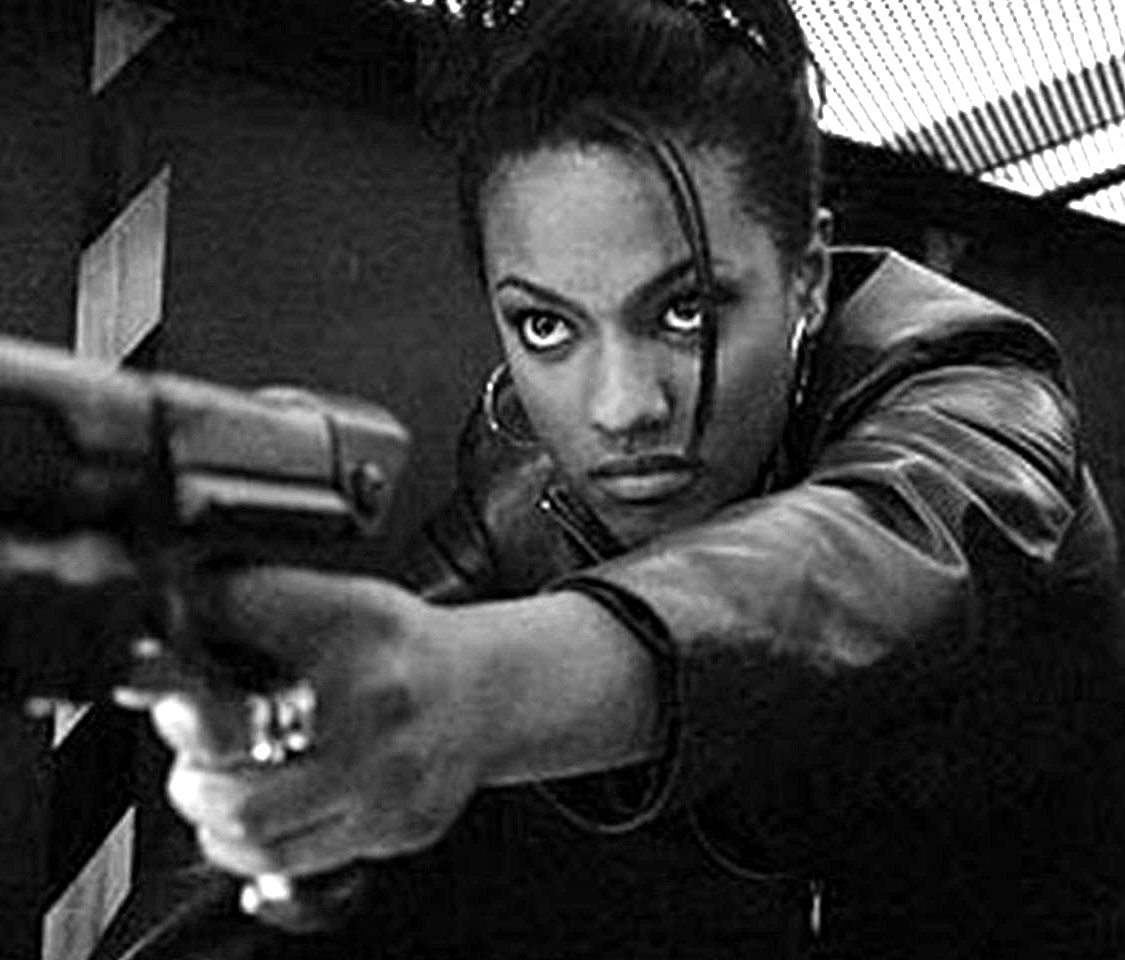
\includegraphics[width=0.2\columnwidth]{pictures/martha} \\

	\parbox{0.3\textwidth}{\center\large The Rebels - try to do it in the fewest parsecs!} &
	\parbox{0.3\textwidth}{\center\large The Pioneers -  } &
	\parbox{0.3\textwidth}{\center\large The Companions - } \\
\end{tabular}
\vspace{5mm}

These items can be submitted to the Front Desk for Fun Points (after 11am).
Pictures are not (generally) admissible; objective involving people {\textit
must only be undertaken with the other person's permission}.
The front desk reserves the right to keep the submitted items. Each faction may
claim an item on the only once, unless otherwise noted.
\begin{tabbing}
	FD \quad \= Front Desk Person's Discretion\footnotemark \\
	E \> This item may be claimed multiple times per faction (``each'') \\
	M \> For each faction, the highest of their scores will be used
\end{tabbing}
\footnotetext{This actually
	applies to everything; where it is noted, it indicates that you’re
	unlikely to change anyone's mind with your cunning arguments.}

\begin{multicols}{2}
	\begin{tabbing}
1 \hspace{12mm}	\= Little Green Pygmy Solders (E) \\
1	\> Hugs (Per person) \\
30	\> Picocon \\
20	\> A non-ICSF fresher at Picocon \\
Age +5	\> Ex-ICSF Chair (M) \\
Age +5	\> Ex-ICSF Librarian (M) \\
Age +5	\> T-shirts from Picocons past (M) \\
10 	\> Previous Guest of Honour (E) \\
10	\> Half of one (1) Dave \\
20	\> The Mabbott set \\
8	\> A Phylactery \\
80 	\> Dave Clements' phylactery \\
100	\> The Picocon Sofa, Calm \\
50	\> The Picocon Beanbag, Frantic \\
15	\> Tea, Earl Grey, Hot \\
25 	\> A good drink (FD, E) \\
10 	\> A less good drink (FD) \\
-5	\> Unsatisfactory drink (FD) \\
5	\> Delicious Blood (FD) \\
15	\> Spirits from beyond \\
1000 	\> £100 (E) \\
7	\> The contents of my pocketses \\
5	\> Good News (FD, E) \\
-5	\> Bad News (FD, E) \\
1	\> A funny joke (FD, E) \\
-1	\> A bad pun (FD, E) \\
25	\> A competent barbershop \\ \> quartet (FD) \\
5	\> Any song sung in the style of \\ \> William Shatner \\
50	\> A barbershop quartet in the style \\ \> of William Shatner \\
50 \> Any door to London Below \\
3   \> Newly acquired merchandise  \\
5   \> A teleological proof of the\\ \> existence of a higher power \\
1   \> The solution to the next item \\ \> on the list (E) \\
-1  \> The solution to the previous \\ \> item on the list (E)\\
10  \> Donations of a themed plastic \\ \> abomination \\
5   \> A demon bear (bonus points if fluffy) \\
5   \> A member of the Family of Blood \\
5   \> A little fall of rain \\
5	\> Origami \\
20  \> Dinosaur Origami \\
10  \> Harmless Victor \\
8	\> A Non-Euclidean Triangle \\
5   \> A snake eating its own snake tail, \\ \> or snail.\\
5	\> Tribble \\
60	\> Tribble (Functional) \\
5	\> A Nanosecond \\
10  \> An accretion disk \\
30  \> A terrifying technological terror \\
3	\> A good hat \\
5	\> A correctly fitted top hat \\
5   \> Convincing closet cosplay \\
10  \> Convincing actual cosplay \\
10  \> Pretty trinkets (FD) \\
3   \> The start of something beautiful \\
30   \> The phone from a castle \\
20  \> The phone from a police box \\
50	\> Happiness, $\ge$ 0.1M Concentration \\
n(n-1)	\> n Interlocking Cogs (Functional \\ \> after being poked) (M) \\
10   \> Out of place kerning \\
20   \> An unaired TV pilot \\
20   \> An untelevised air pilot \\
30 	\> A control crystal (with \\ \> demonstration) \\
40 	\> Three quarters of a planck length \\
20 	\> A demonstration of Xeno's paradox \\
10  \> An aesthetically pleasing key (FD)\\
14 	\> A clowder of one cat \\
5   \> The man they call Jayne (or his hat) \\
-50 \> The source of the mysterious ticking noise \\
400	\> The World Turtle \\
800 \> With orbiting bodies \\
10  \> A surviving member of the Imperial \\ \> Steampunk Society \\
50	\> A book ICSF lacks (and wants) \\
1	\> The Light at the end of the tunnel \\
5	\> A Crowning moment of awesome \\
17	\> Proof Humanity’s reach extends \\ \> beyond its imagination \\
70  \> A lost Dr Who episode \\
3	\> Famous last words (subject to \\ \> checking) \\
-1	\> Anything irrelevent (E) \\
-5  \> Anything irrelephant (E) \\
4   \> A huge Mulligan \\
3	\> Galaxy \\
2	\> A practical application for \\ \> General Relativity \\
4	\> Transcendent understanding \\
10	\> A point in the complex plane \\
30	\> 4 Unitless Sergeis \\
5   \> A working AI (demonstrated) \\
10  \> A working AI (safely demonstrated) \\
1000	\> Time machine (points were awarded \\ \> 17th Feb 6pm, ICSF Library, \\ \> password is ``Apep'') \\
25	\> A swordfish \\
35	\> A fishsword \\
10	\> A Swan \\
4	\> Nerf Guns \\
3	\> NERV guns \\
10	\> Lab Stuff \\
-50	\> per fatality \\
10	\> The Staff of Ra \\
3	\> Positronic Brain \\
3	\> Observable Brownian Motion \\
5	\> A fluffy dragon \\
7	\> A plasma generator \\
5	\> Ion cannon (demonstrated) \\
-20	\> Spontaneous combustion \\ \> whilst dancing (E)\\
5	\> A Henry (E)\\
10	\> A Wild Henry\\
10	\> A completed nonogram (E)\\
15	\> A completed crossword  (E)\\
	\end{tabbing}
\end{multicols}

{\large Good Luck!}

You're likely to need it...
